\subsection{Wood Beams}

\subsubsection{Flexular Stress}

Considering wood as a fibre composite, the flexular strength may be defined as
the stress on the surface of a specimen at a failure, accompanied by the
fracturing of fibers
\cite[chapter 7.2]{hodgikinson-mech-testing-fibre-composites}.

%\begin{figure}[h]
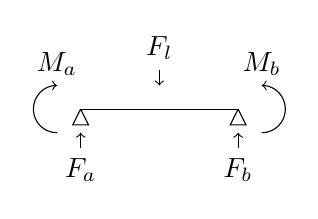
\begin{tikzpicture}
%\draw[help lines, step=0.5] (0, 0) grid (3,2);

\pgfmathsetmacro\baseline{1};
\pgfmathsetmacro\xA{0.5};
\pgfmathsetmacro\xB{3-0.5};
\pgfmathsetmacro\pinHeight{0.2};
\pgfmathsetmacro\arrowLength{0.2};

\draw (\xA, 1) to (\xB, 1);

% triangles
\draw
  (\xA, \baseline) to
  (\xA+\pinHeight/2, \baseline-\pinHeight) to
  (\xA-\pinHeight/2, \baseline-\pinHeight) to
  (\xA, \baseline);

\draw
  (\xB, \baseline) to
  (\xB+\pinHeight/2, \baseline-\pinHeight) to
  (\xB-\pinHeight/2, \baseline-\pinHeight) to
  (\xB, \baseline);

% force
\draw [ -> ]
  (\xA/2 + \xB/2, \baseline + \arrowLength + 1.5*\pinHeight)
    node [above] {$F_l$} to
  (\xA/2 + \xB/2, \baseline + 1.5*\pinHeight);

% reactant forces
\draw [ -> ]
  (\xA, \baseline - \arrowLength - 1.5*\pinHeight)
    node [below] {$F_a$} to
  (\xA, \baseline - 1.5*\pinHeight);

\draw [ -> ]
  (\xB, \baseline - \arrowLength - 1.5*\pinHeight)
    node [below] {$F_b$} to
  (\xB, \baseline - 1.5*\pinHeight);

% moments
\draw [ -> ]
  (\xA - 1.5*\pinHeight, \baseline - 1.5*\pinHeight)
    to [out=-180, in=-90]
  (\xA - 3*\pinHeight, \baseline) to [out=90, in=180]
  (\xA - 1.5*\pinHeight, \baseline + 1.5*\pinHeight)
    node [above] {$M_a$};

\draw [ -> ]
  (\xB + 1.5*\pinHeight, \baseline - 1.5*\pinHeight)
    to [out=0, in=-90]
  (\xB + 3*\pinHeight, \baseline) to [out=90, in=0]
  (\xB + 1.5*\pinHeight, \baseline + 1.5*\pinHeight)
    node [above] {$M_b$};

\end{tikzpicture}
%\caption{Information to the figure}
%\end{figure}

For a bending moment $M$, a width of $b$ and a height of $h$ one may define
the maximum normal stress $\sigma$ as presented in equation
\ref{eq:max-normal-stress}.

\begin{equation}\label{eq:max-normal-stress}
\sigma = \frac{6M}{bh^2}
\end{equation}

With $F_s$ representing the shear force on the cross-section, the maximum shear
stress is presented in equation \ref{eq:max-shear-stress}.

\begin{equation}\label{eq:max-shear-stress}
\tau = \frac{3F_s}{2bh}
\end{equation}

The allowable flexure stress $F'_b$ of wood is tabulated in catalogs, taken
duration $C_D$, moisture $C_M$, beam stablity $C_L$, size $C_F$,
flat use $C_{fu}$ and repetitive member $C_r$ factors into account to define
the flexure as a function of those factors.

\begin{equation}
F'_{b} = F_b(\mathbf C)
\end{equation}

The actual flexure stress is on a wooden beam can be calculated by:

\begin{equation}
f_b = \frac{Mc}{I} = \frac{M}{S} \Biggm\lvert S = \frac{I}{c} = \frac{bd^2}{6}
\end{equation}

\subsubsection{Shear Stress}
The allowable shear stress
